\usetikzlibrary{arrows.meta}
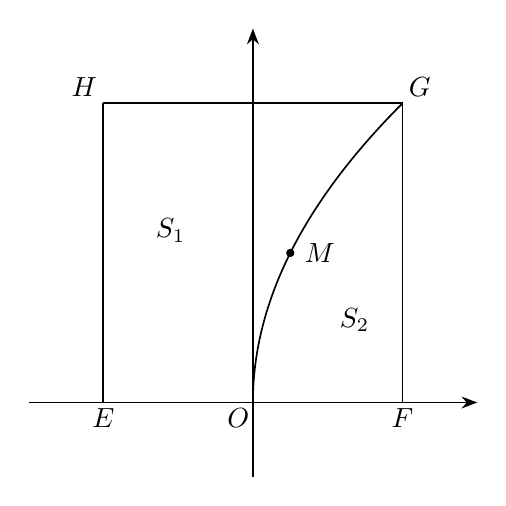
\begin{tikzpicture}[x=1.9cm,y=1.9cm,line width=.6pt,>=Stealth,font=\normalsize,
  axis/.style={line width=.6pt},
  edge/.style={line width=.6pt}]
\coordinate (O) at (0,0);
\coordinate (E) at (-1,0);
\coordinate (F) at (1,0);
\coordinate (H) at (-1,2);
\coordinate (G) at (1,2);
\coordinate (M) at (0.25,1);
\draw[axis,->] (-1.5,0)--(1.5,0);
\draw[axis,->] (0,-0.5)--(0,2.5);
\draw[edge] (E)--(H);
\draw[edge] (H)--(G);
\draw[edge] (G)--(F);
\draw[edge] plot[domain=0:2,samples=101] ({(\x*\x)/4},\x);
\fill (M) circle (1.5pt);
\node[above left,inner sep=0pt,xshift=-2pt,yshift=2pt] at (H) {$H$};
\node[above right,inner sep=0pt,xshift=2pt,yshift=2pt] at (G) {$G$};
\node[below,inner sep=0pt,yshift=-2pt] at (E) {$E$};
\node[below,inner sep=0pt,yshift=-2pt] at (F) {$F$};
\node[below left,inner sep=0pt,xshift=-1pt,yshift=-2pt] at (O) {$O$};
\node[right,inner sep=0pt,xshift=5pt] at (M) {$M$};
\node at (-0.55,1.15) {$S_1$};
\node at (0.68,0.55) {$S_2$};
\end{tikzpicture}
